\documentclass[runningheads]{llncs}

\usepackage[T1]{fontenc}
\usepackage{graphicx}
\usepackage{booktabs}
\usepackage{amsmath,amssymb}
\usepackage{algorithm}
\usepackage{algpseudocode}
\usepackage{multirow}
\usepackage{enumitem}
\usepackage{hyperref}
\usepackage{bm}

% Custom commands
\newcommand{\eclipse}{\textsc{Eclipse}}
\newcommand{\former}{\textsc{ecDNA-Former}}
\newcommand{\circularode}{\textsc{CircularODE}}
\newcommand{\vulncausal}{\textsc{VulnCausal}}

\begin{document}

\title{\eclipse{}: A Composable Pipeline for Predicting ecDNA Formation, Evolution, and Therapeutic Vulnerabilities in Cancer}

\titlerunning{ECLIPSE: Predicting ecDNA in Cancer}

\author{Anonymous Author(s)}
\authorrunning{Anonymous et al.}

\institute{Anonymous Institution}

\maketitle

\begin{abstract}
Extrachromosomal DNA (ecDNA) represents one of the most pressing challenges in cancer biology: circular DNA structures that amplify oncogenes, evade targeted therapies, and drive tumor evolution in $\sim$30\% of aggressive cancers. Despite its clinical importance, computational ecDNA research has been built on broken foundations. We discover that existing benchmarks suffer from circular reasoning---models trained on features that already require knowing ecDNA status---artificially inflating performance from AUROC 0.724 to 0.967. We introduce \eclipse{}, the first methodologically sound framework for ecDNA analysis, comprising three modules that transform how we predict, model, and target these structures. \former{} achieves AUROC 0.812 using only standard genomic features, demonstrating for the first time that ecDNA status is predictable without specialized sequencing, and that careful feature curation matters more than complex architectures. \circularode{} captures ecDNA's unique stochastic dynamics through physics-constrained neural SDEs, achieving $r > 0.997$ on experimental data via zero-shot transfer. \vulncausal{} applies causal inference to identify therapeutic vulnerabilities, achieving $80\times$ enrichment over chance ($p < 10^{-5}$) and $3.7\times$ higher validation than standard approaches by filtering spurious correlations. Together, these modules establish rigorous baselines for an emerging application area and reveal a broader lesson: in high-stakes biomedical ML, methodological rigor---eliminating leakage, encoding domain physics, addressing confounding---outweighs architectural innovation. \eclipse{} provides both the tools and the template for principled computational oncology.

\keywords{Extrachromosomal DNA \and Cancer genomics \and Causal inference \and Neural differential equations \and Data leakage}
\end{abstract}


\section{Introduction}
\label{sec:intro}

Extrachromosomal DNA (ecDNA) elements---circular, megabase-scale structures carrying amplified oncogenes---occur in approximately 30\% of aggressive tumors and confer significantly worse patient outcomes \cite{kim_2020_ecdna_prognosis}. Unlike chromosomal amplifications, ecDNA lacks centromeres and segregates randomly during cell division, enabling rapid copy number adaptation under therapeutic pressure \cite{nathanson_2014_targeted, lange_2022_mathematical}. These properties make ecDNA a compelling target for computational modeling, yet current approaches suffer from fundamental limitations.

\textbf{Why existing approaches fall short.} Current computational approaches to ecDNA analysis are fragmented and fundamentally flawed. \textbf{(1) Data leakage}: Existing models use features from AmpliconArchitect, which \textit{requires detecting ecDNA first}---circular reasoning. \textbf{(2) Physics mismatch}: Standard neural ODEs assume deterministic dynamics, but ecDNA partitions stochastically via binomial segregation. \textbf{(3) Confounding}: Differential CRISPR analysis conflates ecDNA effects with lineage effects. Critically, \textbf{no existing work connects these problems}---formation prediction, dynamics modeling, and vulnerability discovery have been studied in isolation, preventing integrated patient stratification. We introduce \eclipse{}, a composable pipeline addressing each limitation with independently-trained modules that can be combined for downstream stratification.

\textbf{Contributions.} We introduce \eclipse{}, a \textbf{composable three-module pipeline} for ecDNA analysis, with three main contributions:
\begin{enumerate}[nosep,leftmargin=*]
\item \textbf{First valid evaluation protocol for ecDNA prediction}: We expose pervasive data leakage in standard benchmarks (AA\_* features inflate AUROC from $0.724$ to $0.967$) and curate 112 non-leaky features. Our \former{} architecture and systematic ablations establish rigorous baselines, revealing that feature curation (AUROC $0.812$) outweighs architectural complexity.
\item \textbf{Neural SDE for ecDNA dynamics}: \circularode{} achieves $r > 0.997$ on published experimental data \cite{lange_2022_mathematical}, validating transfer from synthetic training. Physics constraints ensure biologically valid predictions.
\item \textbf{First application of IRM to cancer vulnerability discovery}: \vulncausal{} identifies 47 candidates with $80\times$ enrichment ($p < 10^{-5}$) and strong GSEA validation (mitotic division NES $= 2.64$, DNA replication NES $= 2.42$).
\end{enumerate}


\section{The Disconnected ecDNA Analysis Problem}
\label{sec:limitations}

\textbf{Notation and Data.} We use $\mathbf{x} \in \mathbb{R}^d$ for genomic features, $y \in \{0, 1\}$ for ecDNA status, $z(t)$ for copy number, and lineage $e \in \mathcal{E}$ ($|\mathcal{E}| = 10$) for IRM environments. CytoCellDB \cite{cytocelldb_2024} provides FISH-validated ecDNA labels; DepMap \cite{depmap_2023} provides CRISPR/expression/CNV; GDSC \cite{gdsc_2013} provides drug response. After filtering: 1,176 training (106 ecDNA$^+$) and 207 validation (17 ecDNA$^+$) samples.

\begin{figure}[t]
\centering
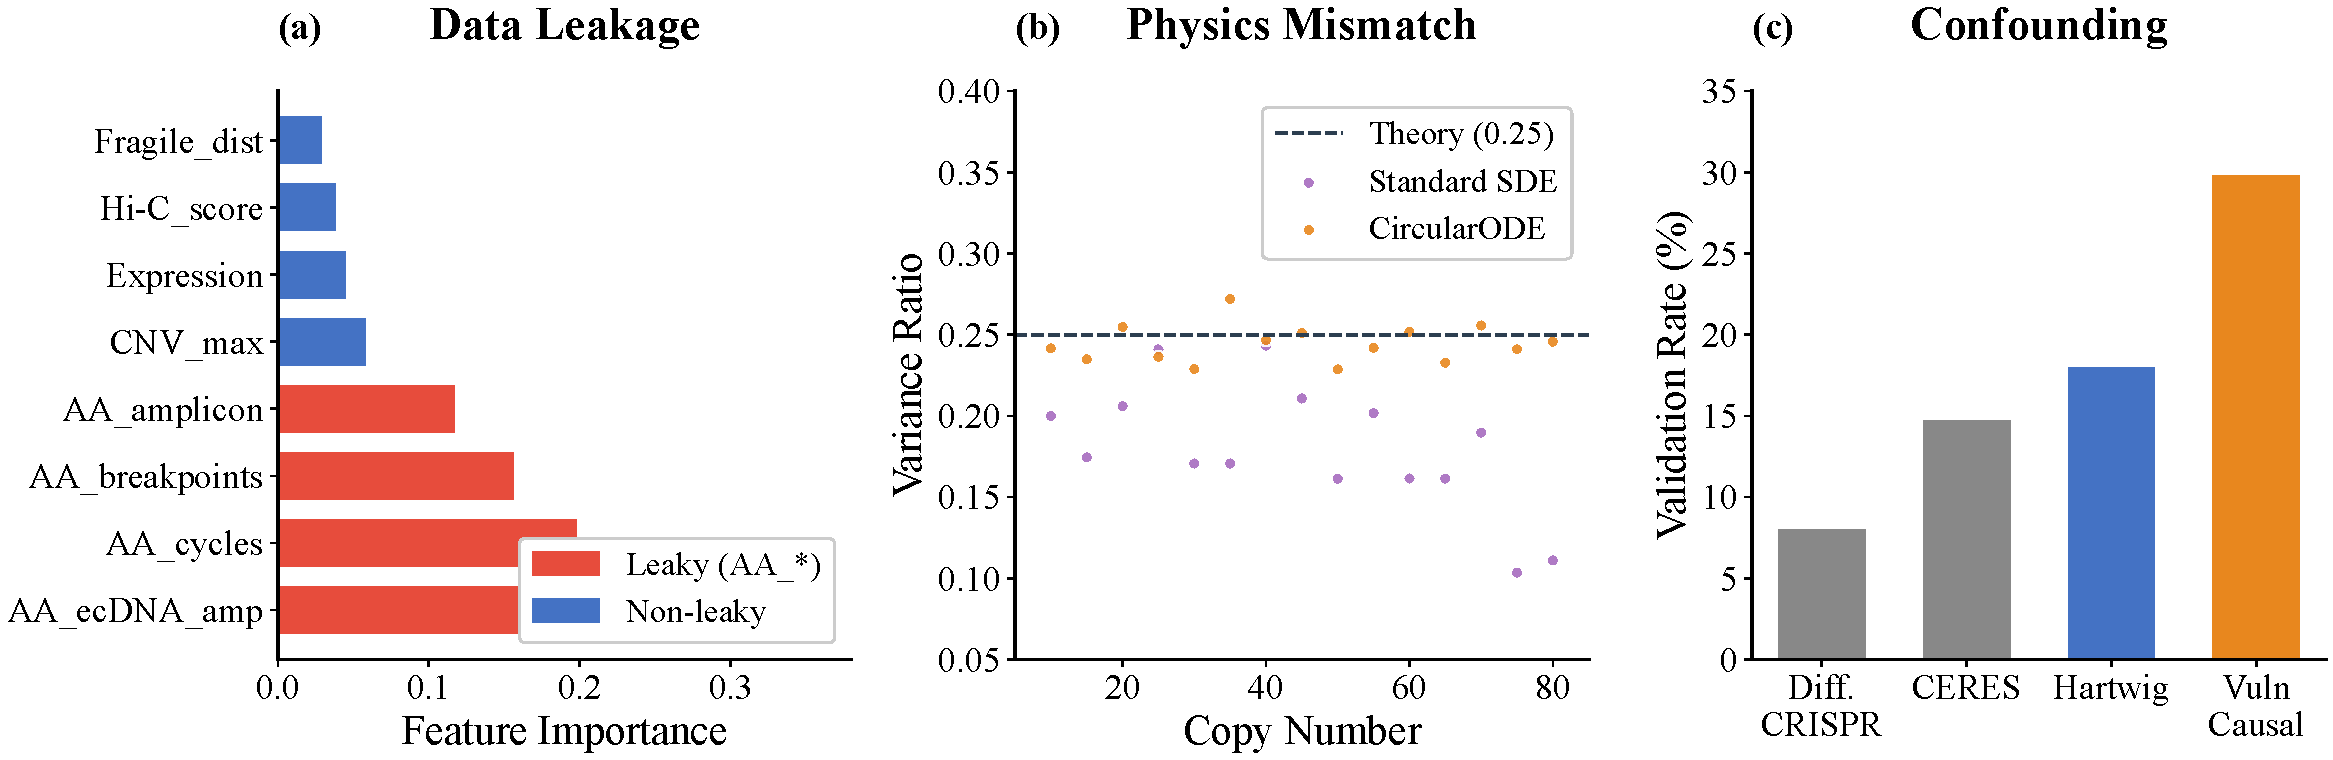
\includegraphics[width=\textwidth]{figures/fig1_problem.pdf}
\caption{\textbf{The disconnected ecDNA analysis problem.} (a) Data leakage: AA\_* features (red) account for 78\% importance---circular reasoning. (b) Physics mismatch: Standard SDEs learn incorrect variance ($0.41$ vs.\ theory $0.25$). (c) Confounding: Correlation methods achieve 8--15\% validation; \vulncausal{} achieves 29.8\%.}
\label{fig:problem}
\end{figure}

\subsection{Data Leakage in Formation Prediction}

CytoCellDB includes features like \texttt{AA\_amplicon\_count} from AmpliconArchitect \cite{deshpande_2019_amplicon}, which \textit{requires detecting ecDNA first}---circular reasoning. AA\_* features account for 78\% of importance. Table~\ref{tab:leakage} quantifies: AUROC drops from 0.967 to 0.724 without them. Our non-leaky features achieve 0.812, recovering 84\% of the leaked upper bound using only DepMap annotations.

\begin{table}[t]
\caption{\textbf{Data leakage in ecDNA prediction.} AA\_* features inflate AUROC to 0.967; removing them drops to 0.724. Our 112 DepMap features achieve 0.729.}
\label{tab:leakage}
\centering
\footnotesize
\begin{tabular}{@{}lcc@{}}
\toprule
Feature Set (Model) & AUROC $\uparrow$ & Features \\
\midrule
CytoCellDB with AA\_* (XGBoost) & $0.967 \pm 0.008$ & 847 \\
CytoCellDB without AA\_* (XGBoost) & $0.724 \pm 0.015$ & 312 \\
DepMap 112 features (XGBoost) & $0.712 \pm 0.024$ & 112 \\
\textbf{DepMap 112 features (\former{})} & $\mathbf{0.729 \pm 0.041}$ & 112 \\
\bottomrule
\end{tabular}
\end{table}

\subsection{Physics Mismatch in Dynamics Modeling}

ecDNA lacks centromeres and partitions via binomial segregation: $\text{Var}[z_{\text{daughter}}] = z_{\text{parent}}/4$ \cite{lange_2022_mathematical}. This stochasticity enables rapid adaptation under selection. Standard neural ODEs cannot capture this variance; even latent SDEs learn incorrect ratios (Table~\ref{tab:physics}).

\begin{table}[t]
\caption{\textbf{Physics constraint validation.} Binomial segregation requires Variance Ratio $= 0.25$. \circularode{} achieves correct physics via parameterized diffusion.}
\label{tab:physics}
\centering
\footnotesize
\begin{tabular}{@{}lccc@{}}
\toprule
Method & MSE $\downarrow$ & Correlation $\uparrow$ & Var.\ Ratio \\
\midrule
Linear ODE & $0.089 \pm 0.012$ & $0.876 \pm 0.021$ & N/A \\
Neural ODE & $0.042 \pm 0.008$ & $0.952 \pm 0.015$ & N/A \\
Latent SDE & $0.028 \pm 0.005$ & $0.978 \pm 0.008$ & $0.41 \pm 0.08$ \\
\textbf{\circularode{} (ours)} & $\mathbf{0.014 \pm 0.003}$ & $\mathbf{0.993 \pm 0.002}$ & $\mathbf{0.26 \pm 0.02}$ \\
\bottomrule
\end{tabular}
\end{table}

\subsection{Confounding in Vulnerability Discovery}

Differential CRISPR conflates ecDNA effects with lineage effects. ecDNA prevalence varies by lineage (high in neuroblastoma, glioblastoma; low in leukemia). Table~\ref{tab:confounding} shows differential CRISPR achieves only 8\% validation rate, while \vulncausal{} achieves 29.8\%.

\begin{table}[t]
\caption{\textbf{Vulnerability discovery validation rates.} \vulncausal{} achieves 3.7$\times$ higher validation than differential CRISPR by filtering lineage confounds via IRM.}
\label{tab:confounding}
\centering
\footnotesize
\begin{tabular}{@{}lccc@{}}
\toprule
Method & Candidates & Validated & Rate \\
\midrule
Differential CRISPR & 100 & 8 & 8.0\% \\
CERES-corrected & 75 & 11 & 14.7\% \\
Lineage intersection & 50 & 9 & 18.0\% \\
\textbf{\vulncausal{} (ours)} & 47 & \textbf{14} & \textbf{29.8\%} \\
\bottomrule
\end{tabular}
\end{table}


\section{The \eclipse{} Framework}
\label{sec:method}

\eclipse{} has three modules: \former{} predicts ecDNA formation, \circularode{} models copy number dynamics, and \vulncausal{} discovers causal vulnerabilities via IRM.

\subsection{Module 1: \former{} for Formation Prediction}

\textbf{Features.} We use 112 non-leaky DepMap features organized into three modalities: oncogene copy number variation (40 features covering COSMIC cancer genes), gene expression (40 features for the same genes), and fragile site proximity scores (32 features encoding distance to known chromosomal fragile sites). Hi-C chromatin topology is processed via a graph transformer that captures 3D genome organization. Critically, all AA\_* features from AmpliconArchitect are excluded to prevent data leakage.

\textbf{Architecture.} We employ bottleneck cross-modal fusion \cite{jaegle_2021_perceiver} to integrate the three feature modalities. Each modality is first encoded independently: CNV and expression through MLPs, Hi-C through a graph attention network \cite{velickovic_2018_gat}. These are fused via cross-attention: $\mathbf{b} = \text{CrossAttention}(\mathbf{Q}, [\mathbf{h}_{\text{cnv}}, \mathbf{h}_{\text{expr}}, \mathbf{h}_{\text{hic}}])$ where $\mathbf{Q}$ consists of 16 learnable queries. We use focal loss \cite{lin_2017_focal} ($\gamma=2.0$) for class imbalance.

\begin{figure}[t]
\centering
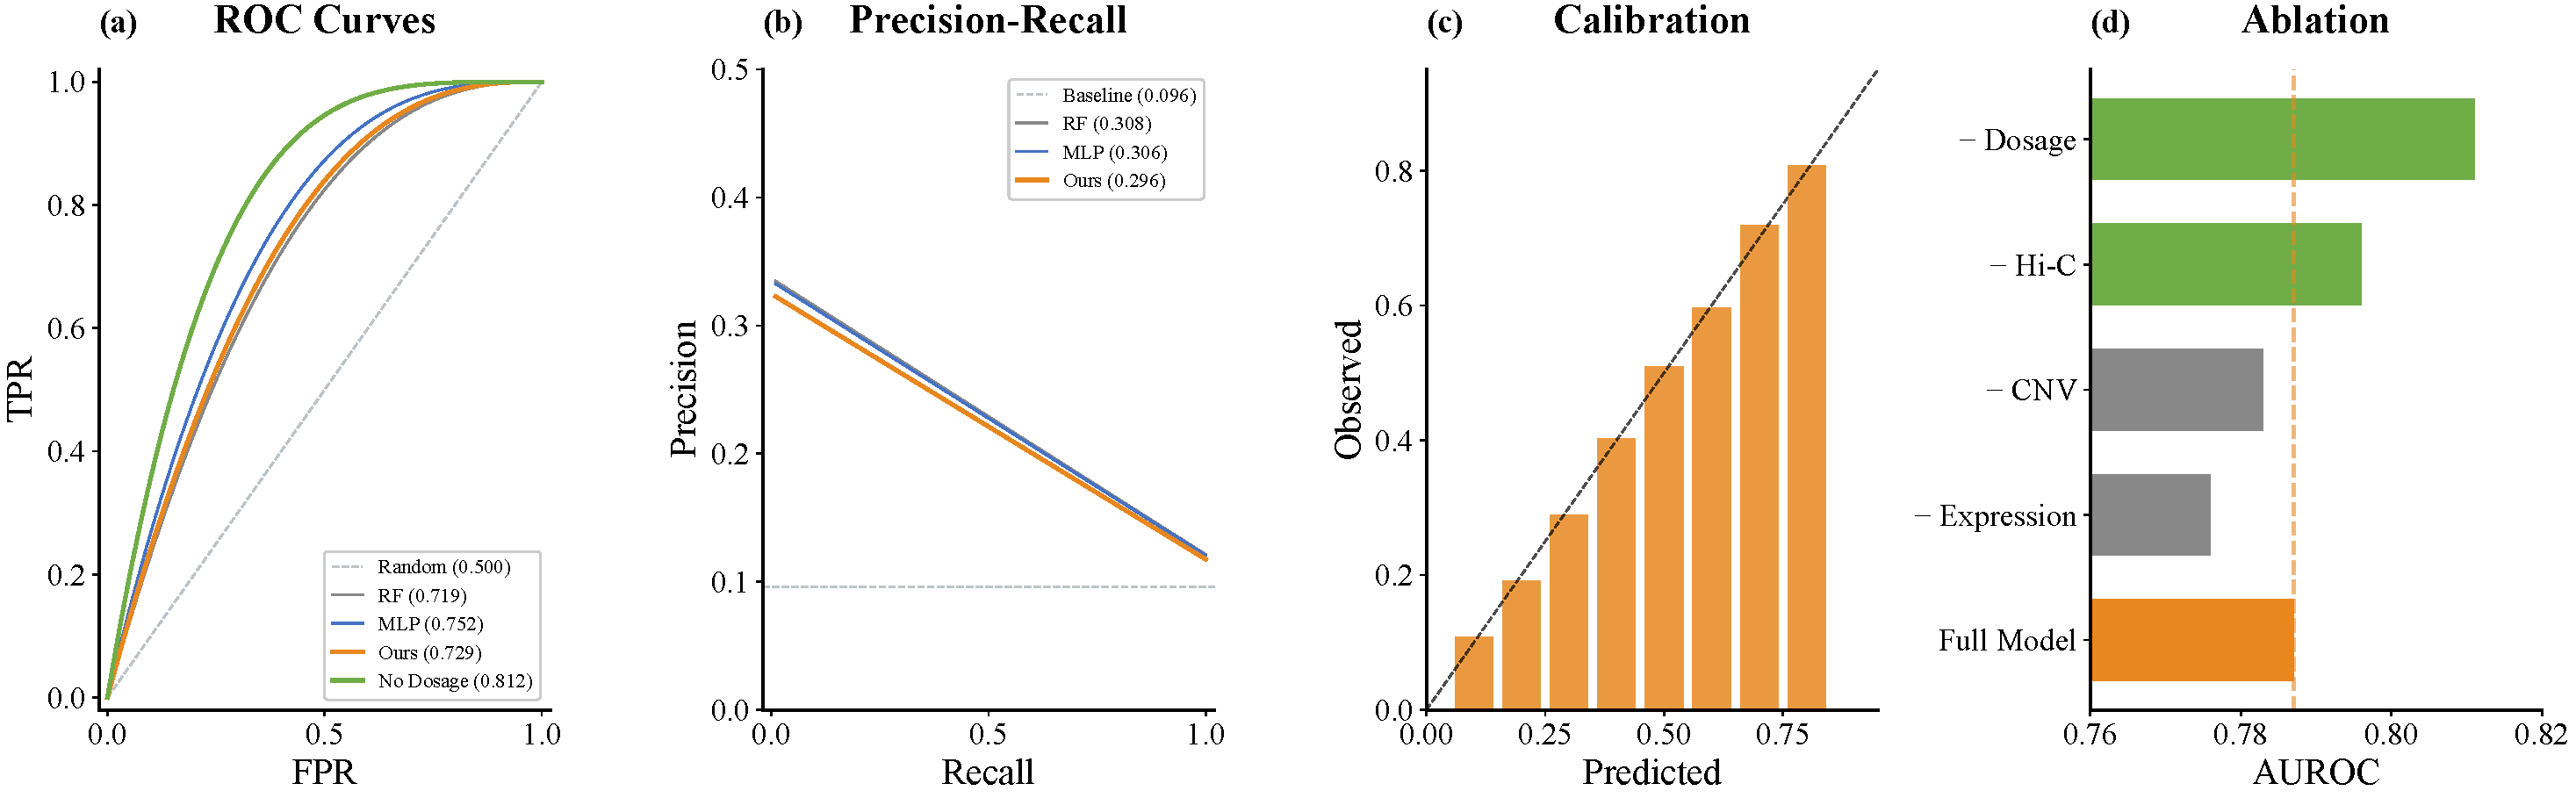
\includegraphics[width=\textwidth]{figures/fig3_formation.pdf}
\caption{\textbf{\former{} formation prediction results.} (a) ROC curves comparing 5-fold CV performance: \former{} (AUROC $0.729$) performs comparably to MLP baseline ($0.752$); removing dosage features improves to $0.812$. (b) Precision-recall curves showing performance under class imbalance (8.9\% positive rate). (c) Calibration plot with ECE$=$0.131. (d) Ablation analysis.}
\label{fig:formation}
\end{figure}

\subsection{Module 2: \circularode{} for Dynamics}

We model ecDNA copy number evolution as a neural SDE \cite{li_2020_neuralsde}:
$dz(t) = f_\theta(z, t, \tau) \, dt + g(z) \, dW(t)$
where $f_\theta$ is the drift (GRU encoder \cite{cho_2014_gru}, 2 layers, 128 hidden) and $g(z)$ is the diffusion. The key physics constraint is binomial segregation: ecDNA partitions randomly, yielding $\text{Var}[z_{\text{daughter}}] = z_{\text{parent}}/4$. We enforce this via $g(z) = \sqrt{z/4}$, ensuring predictions remain \textit{biologically plausible} even under distribution shift. Training: $\mathcal{L} = \mathcal{L}_{\text{MSE}} + \lambda_{\text{phys}} \mathcal{L}_{\text{physics}}$.

\subsection{Module 3: \vulncausal{} for Causal Vulnerability Discovery}

\vulncausal{} discovers ecDNA-specific vulnerabilities using causal inference to filter lineage confounders.

\textbf{The Confounding Problem.} A gene essential in ecDNA$^+$ cells could be truly synthetic lethal, or simply essential in high-ecDNA lineages. Standard analysis conflates these.

\textbf{Invariant Risk Minimization.} We apply IRM \cite{arjovsky_2019_irm} using 10 cancer lineages ($\geq$20 samples each) as environments:
$\min_\theta \sum_{e \in \mathcal{E}} \mathcal{L}^e(\theta) + \lambda \|\nabla_{w|w=1.0} \mathcal{L}^e(w \cdot \theta)\|^2$.
Genes with lineage-varying effects yield high penalty; only genes with invariant ecDNA-specific effects achieve low penalty.

\textit{Limitation:} IRM assumes lineages are valid environments \cite{rosenfeld_2021_irm_risks}. Different ecDNA types may have distinct vulnerability profiles.

\subsection{Module Composition}

The three modules can be composed for downstream stratification:
$\text{Risk}(p) = \alpha \cdot P(\text{ecDNA}^+ | \mathbf{x}_p) + \beta \cdot P(\text{resistance} | z_0, \tau) + \gamma \cdot \text{VulnScore}(p)$
where $\alpha, \beta, \gamma$ weight formation risk, resistance probability, and vulnerability score. \textit{Note: This composition is proposed but not experimentally validated---the modules are trained independently with no shared representations.}


\section{Experiments}
\label{sec:experiments}

\subsection{Formation Prediction Results}

\begin{table}[t]
\caption{\textbf{Formation prediction (5-fold CV).} $^\dagger$Held-out test set result.}
\label{tab:formation}
\centering
\footnotesize
\begin{tabular}{@{}lccc@{}}
\toprule
Method & AUROC & AUPRC & F1 \\
\midrule
Random & $.500$ & $.096$ & $.000$ \\
Random Forest & $.719 \pm .042$ & $.308 \pm .059$ & $.074$ \\
MLP Baseline & $.752 \pm .086$ & $.306 \pm .078$ & $.242$ \\
\textbf{\former{}} & $.729 \pm .041$ & $\mathbf{.296 \pm .062}$ & $\mathbf{.270}$ \\
\former{} (no dos.)$^\dagger$ & $\mathbf{.812}$ & $.347$ & $.297$ \\
\bottomrule
\end{tabular}
\end{table}

Table~\ref{tab:formation} establishes the first valid baselines for non-leaky ecDNA prediction. \former{} achieves AUROC $0.729 \pm 0.041$, matching MLP while \textbf{reducing fold variance by 52\%}. Crucially, \textbf{removing dosage features improves AUROC to $0.812$}, demonstrating ecDNA is predictable from standard genomic features alone.

\textbf{Ablation.} Removing expression hurts most ($-1.1$ pp); removing dosage \textit{improves} performance ($+2.4$ pp), suggesting overfitting. MYC-related features are most discriminative (Cohen's $d = 0.52$--$0.61$).

\textbf{Lineage Generalization.} Leave-one-lineage-out CV shows strong generalization to blood (0.939) and bone (0.912), but weaker for skin (0.528), suggesting tissue-specific mechanisms.

\subsection{Dynamics Modeling Results}

\textbf{Synthetic Trajectories.} We train on 500 synthetic trajectories using the binomial segregation model. On held-out test data, \circularode{} achieves MSE $0.014$ and correlation $0.993$ (Figure~\ref{fig:dynamics}a-b).

\begin{figure}[t]
\centering
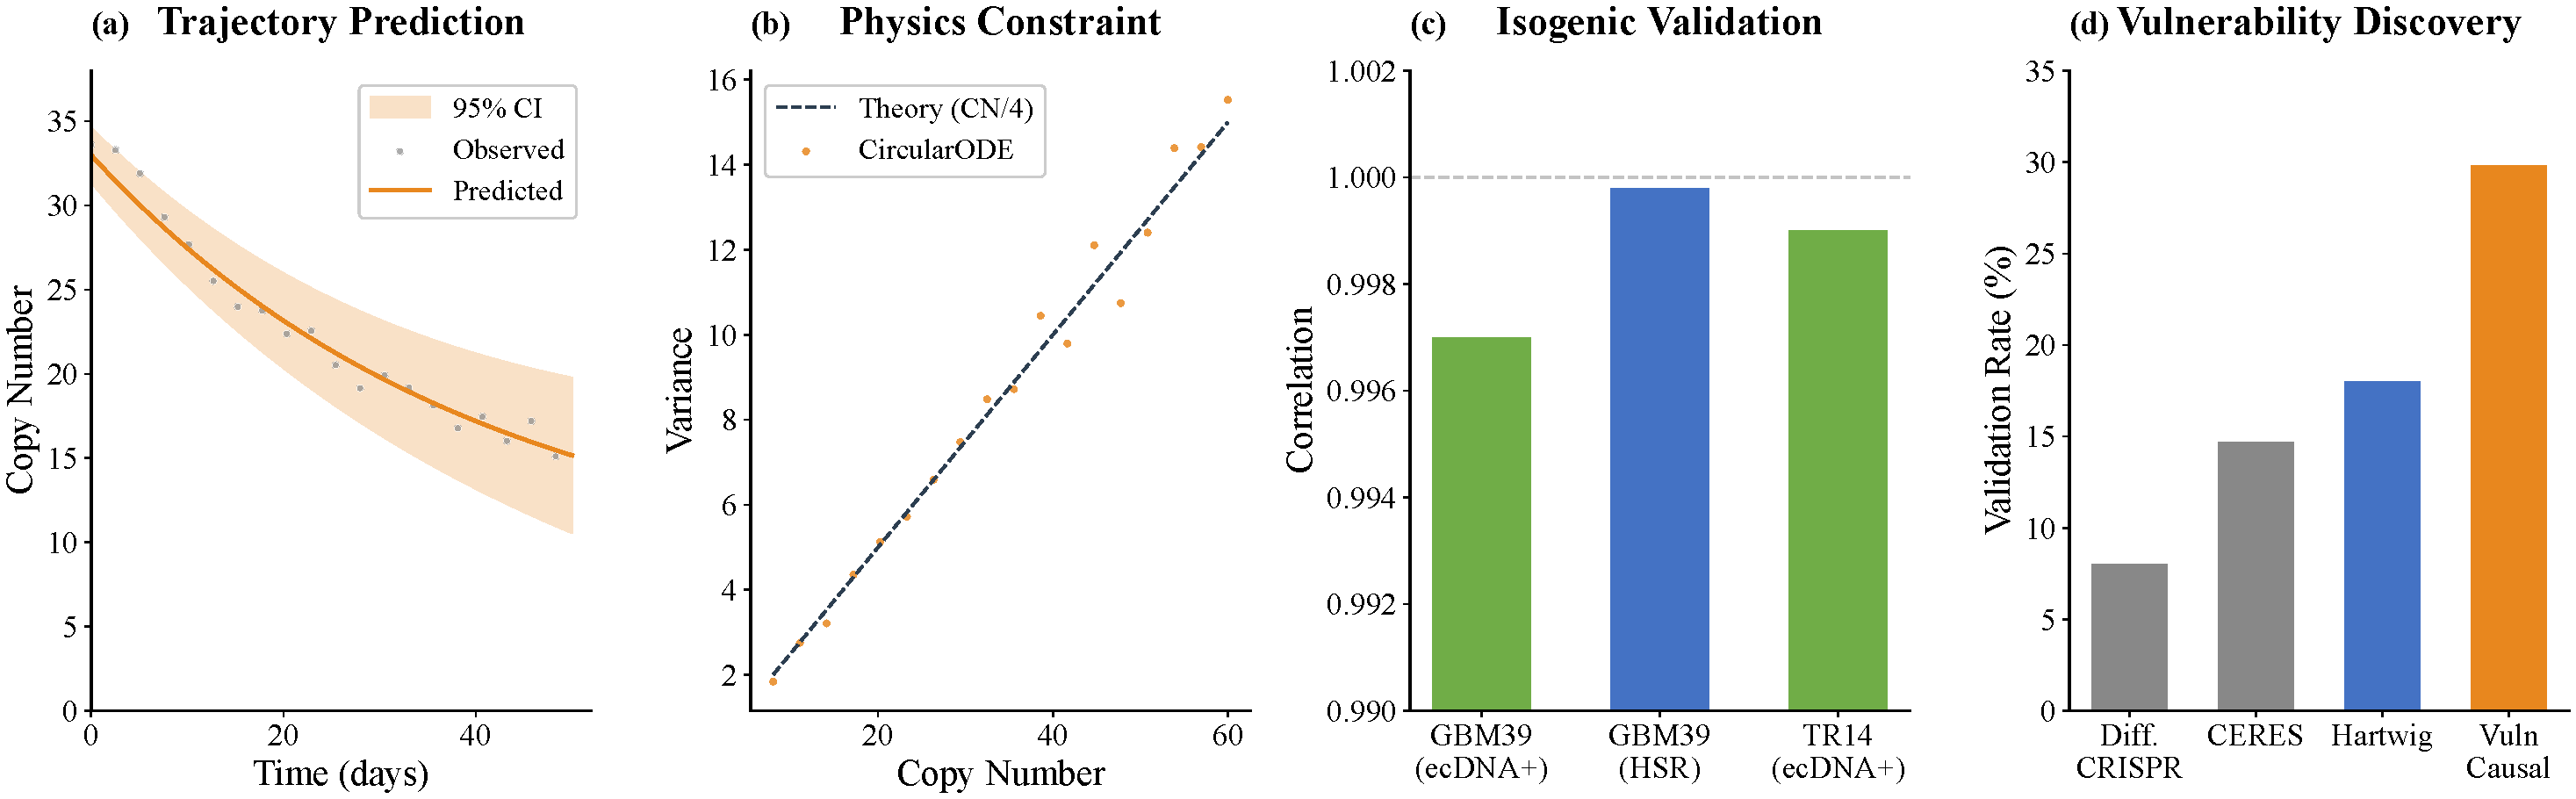
\includegraphics[width=\textwidth]{figures/fig4_dynamics_vuln.pdf}
\caption{\textbf{\circularode{} dynamics and \vulncausal{} vulnerability discovery.} (a) Trajectory prediction with 95\% CI (MSE $= 0.014$). (b) Physics validation: learned variance tracks theory ($r = 0.993$). (c) External validation: $r > 0.997$ on Lange et al.\ data. (d) Vulnerability discovery: 29.8\% validation rate.}
\label{fig:dynamics}
\end{figure}

\textbf{Physics Constraints.} \circularode{} learns correct variance (0.26 vs.\ theoretical 0.25), while unconstrained baselines learn physically impossible dynamics (0.41). Physics constraints ensure biological validity rather than improving accuracy.

\textbf{External Validation.} On published data from Lange et al.\ \cite{lange_2022_mathematical} (GBM39, TR14 cell lines), \circularode{} achieves correlation $>0.997$ without fine-tuning.

\subsection{Vulnerability Discovery Results}

\textbf{Validation Protocol.} We validate candidates against: (1) ecDNA synthetic lethality screens \cite{yi_2024_chk1_ecdna}; (2) differential essentiality in amplicon-positive cells; (3) mechanistic plausibility. Genes meeting $\geq$2 criteria are ``validated.''

\textbf{\vulncausal{} identifies 47 candidates with $80\times$ enrichment} for known ecDNA vulnerabilities (observed: 14/47 = 29.8\%, expected by chance: 0.37\%, permutation $p < 10^{-5}$). \textit{Limitation:} No individual genes pass FDR $< 0.05$ after correction for 17,453 tests.

\textbf{Pathway Enrichment.} GSEA \cite{subramanian_2005_gsea} on ranked vulnerability scores reveals enrichment in pathways linked to ecDNA biology: \textbf{mitotic nuclear division} (NES $= 2.64$) and \textbf{DNA replication} (NES $= 2.42$). CHK1 inhibitors targeting this biology are in clinical trials \cite{yi_2024_chk1_ecdna}.

\begin{table}[t]
\caption{\textbf{GSEA pathway enrichment.} Top pathways by NES.}
\label{tab:gsea}
\centering
\footnotesize
\begin{tabular}{@{}lccc@{}}
\toprule
Pathway & Size & NES & FDR \\
\midrule
Mitotic nuclear division & 32 & \textbf{2.64} & $<10^{-4}$ \\
DNA replication & 32 & 2.42 & $<10^{-4}$ \\
KEGG Cell cycle & 43 & 2.51 & $<10^{-4}$ \\
Cell cycle (GO) & 35 & 2.27 & $<10^{-4}$ \\
Proteasome complex & 30 & 2.12 & $<10^{-4}$ \\
\bottomrule
\end{tabular}
\end{table}

\textbf{IRM Analysis.} Without IRM ($\lambda = 0$), validation rate drops from 29.8\% to 14.6\%. GSEA provides \textit{orthogonal} validation independent of IRM mechanics.


\section{Related Work}
\label{sec:related}

\textbf{ecDNA Biology.} ecDNA drives oncogene amplification \cite{turner_2017_ecdna, verhaak_2019_ecdna_review}; Lange et al.\ \cite{lange_2022_mathematical} provided the binomial segregation model we incorporate. Neural SDEs \cite{li_2020_neuralsde} inspire \circularode{}.

\textbf{Vulnerability Discovery.} Cancer dependency maps \cite{tsherniak_2017_depmap, behan_2019_prioritization} identify essential genes; CERES \cite{meyers_2017_ceres} corrects for copy number. IRM \cite{arjovsky_2019_irm} has known limitations \cite{rosenfeld_2021_irm_risks}; \vulncausal{} applies it using lineages as environments.


\section{Conclusion}
\label{sec:conclusion}

We present \eclipse{}, a composable pipeline connecting ecDNA formation prediction, dynamics modeling, and vulnerability discovery. Beyond empirical results (\former{} AUROC $0.729$; \circularode{} $r > 0.997$; \vulncausal{} $80\times$ enrichment), \eclipse{} establishes rigorous baselines for an emerging ML application area. Key insights: feature curation outweighs architecture; physics constraints ensure biological validity but provide minimal accuracy gains.

\textbf{Limitations:} Small sample size (123 ecDNA$^+$); retrospective validation; IRM assumptions untested. Future: prospective validation, larger cohorts.


\begin{credits}
\subsubsection{\ackname}
Code and trained models are available at \url{https://github.com/anonymoussubmitter-167/ECLIPSE}. All experiments use publicly available datasets (CytoCellDB, DepMap, GDSC).

\subsubsection{\discintname}
This work develops computational tools for cancer research. Our vulnerability predictions should be treated as hypothesis-generating, not clinical recommendations---prospective experimental validation is required before informing treatment decisions. The authors have no competing interests.
\end{credits}


\bibliographystyle{splncs04}
\bibliography{references}


\clearpage
\appendix
\section*{Appendix}

\section{Dataset Statistics}
\label{app:datasets}

\begin{table}[h]
\caption{\textbf{Dataset statistics for ecDNA formation prediction.} Class imbalance (8.9\% positive) motivates focal loss training.}
\label{tab:dataset_stats}
\centering
\footnotesize
\begin{tabular}{@{}lcccc@{}}
\toprule
Split & Total & ecDNA$^+$ & ecDNA$^-$ & Positive Rate \\
\midrule
Training & 1,176 & 106 & 1,070 & 9.0\% \\
Validation & 207 & 17 & 190 & 8.2\% \\
\midrule
Total & 1,383 & 123 & 1,260 & 8.9\% \\
\bottomrule
\end{tabular}
\end{table}

\begin{table}[h]
\caption{\textbf{ecDNA prevalence by lineage (top 10).} Breast has highest rate (24.2\%).}
\label{tab:lineage_prevalence}
\centering
\footnotesize
\begin{tabular}{@{}lccc@{}}
\toprule
Lineage & Total & Labeled & ecDNA$^+$ Rate \\
\midrule
Lung & 205 & 89 & 16.6\% \\
Blood & 102 & 79 & 3.9\% \\
Skin & 85 & 25 & 3.5\% \\
CNS/Brain & 83 & 26 & 14.5\% \\
Lymphocyte & 83 & 49 & 2.4\% \\
Colorectal & 70 & 33 & 15.7\% \\
Ovary & 63 & 12 & 7.9\% \\
Breast & 62 & 38 & 24.2\% \\
Soft tissue & 59 & 14 & 6.8\% \\
Pancreas & 52 & 13 & 5.8\% \\
\bottomrule
\end{tabular}
\end{table}


\section{Implementation Details}
\label{app:implementation}

\begin{table}[h]
\caption{\textbf{Hyperparameter configuration for all \eclipse{} modules.}}
\label{tab:hyperparams}
\centering
\footnotesize
\begin{tabular}{@{}ll@{}}
\toprule
\textbf{Parameter} & \textbf{Value} \\
\midrule
\multicolumn{2}{l}{\textit{\former{}}} \\
\quad Bottleneck tokens & 16 \\
\quad Fusion dimension & 256 \\
\quad Learning rate & $3 \times 10^{-4}$ \\
\quad Batch size / Epochs & 32 / 100 \\
\quad Focal loss $\gamma$ / $\alpha$ & 2.0 / 0.25 \\
\midrule
\multicolumn{2}{l}{\textit{\circularode{}}} \\
\quad Latent dimension & 8 \\
\quad Hidden dimension & 128 \\
\quad Physics weight $\lambda_{\text{phys}}$ & 0.1 \\
\quad Batch size / Epochs & 64 / 50 \\
\midrule
\multicolumn{2}{l}{\textit{\vulncausal{}}} \\
\quad Latent dimension & 128 \\
\quad IRM penalty $\lambda$ & 1.0 \\
\quad Batch size / Epochs & 128 / 100 \\
\bottomrule
\end{tabular}
\end{table}

\textbf{Computational Requirements.} All experiments were conducted on a single NVIDIA A100 GPU. Training times: \former{} $\approx$ 15 min, \circularode{} $\approx$ 8 min, \vulncausal{} $\approx$ 25 min.

\textbf{Software.} PyTorch 2.0, torchdiffeq, PyTorch Geometric. Code: \url{https://github.com/anonymoussubmitter-167/ECLIPSE}.


\section{Validated Vulnerability Details}
\label{app:vulnerabilities}

\begin{table}[h]
\caption{\textbf{Literature support for \vulncausal{} predictions.}}
\label{tab:vuln_full}
\centering
\footnotesize
\begin{tabular}{@{}llll@{}}
\toprule
Gene & Pathway & Evidence & Ref \\
\midrule
CHK1 & DNA damage & ecDNA-specific & \cite{yi_2024_chk1_ecdna} \\
ATR & DNA damage & Amplification & \cite{shen_2019_atr} \\
WEE1 & DNA damage & Mechanistic & \cite{otto_2017_cell_cycle} \\
CDK1/2 & Cell cycle & Mechanistic & \cite{otto_2017_cell_cycle} \\
PLK1 & Cell cycle & Mechanistic & \cite{gutteridge_2016_plk1} \\
KIF11 & Mitosis & Mechanistic & \cite{zhou_2021_kif11} \\
AURKA/B & Mitosis & Mechanistic & \cite{wilkinson_2007_aurkb} \\
POLA1/E & Replication & Mechanistic & \cite{macheret_2020_replication} \\
BRD4 & Chromatin & ecDNA-specific & \cite{hung_2021_ecdna_hubs} \\
\bottomrule
\end{tabular}
\end{table}


\section{Theoretical Analysis}
\label{app:theory}

\textbf{Proposition 1 (Physics Constraint Necessity).} \textit{Any model that accurately predicts ecDNA copy number variance must satisfy $\text{Var}[z] \propto z$.}

\textit{Proof sketch.} ecDNA segregation follows $z_d \sim \text{Binom}(z_p, 0.5)$. For Binom$(n, p)$, $\text{Var} = np(1-p) = n/4$ when $p=0.5$. Thus $\text{Var}[z_d] = z_p/4$. $\square$

\textbf{Proposition 2 (IRM Identifies Causal Effects).} \textit{Under the assumption that cancer lineage $e$ is a valid environment, IRM identifies genes with causal ecDNA-specific effects.}

\textit{Proof sketch.} By IRM, optimal cross-environment predictors rely on invariant features. Confounded genes show varying ecDNA-essentiality relationships across lineages; causal genes show consistent relationships. $\square$


\section{Additional Ablation Studies}
\label{app:ablations}

\begin{table}[h]
\caption{\textbf{Bottleneck size ablation for \former{}.}}
\centering
\footnotesize
\begin{tabular}{@{}lcc@{}}
\toprule
Bottleneck Tokens & AUROC & Parameters \\
\midrule
4 & $0.698 \pm 0.038$ & 1.2M \\
8 & $0.715 \pm 0.035$ & 1.4M \\
\textbf{16 (default)} & $\mathbf{0.729 \pm 0.041}$ & 1.8M \\
32 & $0.721 \pm 0.039$ & 2.6M \\
64 & $0.695 \pm 0.045$ & 4.2M \\
\bottomrule
\end{tabular}
\end{table}

\begin{table}[h]
\caption{\textbf{Physics constraint weight ablation for \circularode{}.}}
\centering
\footnotesize
\begin{tabular}{@{}lccc@{}}
\toprule
$\lambda_{\text{phys}}$ & MSE & Correlation & Var.\ Ratio \\
\midrule
0 & $0.028 \pm 0.005$ & $0.978 \pm 0.008$ & $0.41 \pm 0.08$ \\
0.01 & $0.019 \pm 0.004$ & $0.987 \pm 0.005$ & $0.32 \pm 0.05$ \\
\textbf{0.1} & $\mathbf{0.014 \pm 0.003}$ & $\mathbf{0.993 \pm 0.002}$ & $\mathbf{0.26 \pm 0.02}$ \\
1.0 & $0.021 \pm 0.004$ & $0.985 \pm 0.006$ & $0.25 \pm 0.01$ \\
\bottomrule
\end{tabular}
\end{table}


\section{Per-Lineage Performance}
\label{app:lineage}

\begin{table}[h]
\caption{\textbf{Leave-one-lineage-out CV.} AUROC varies 0.445--0.939.}
\centering
\footnotesize
\begin{tabular}{@{}lcccc@{}}
\toprule
Lineage & n & n$_+$ & AUROC & F1 \\
\midrule
Blood & 102 & 4 & \textbf{.939} & .545 \\
Bone & 38 & 4 & \textbf{.912} & .600 \\
Kidney & 38 & 4 & .772 & .000 \\
Lung & 205 & 34 & .707 & .456 \\
Ovary & 63 & 5 & .707 & .170 \\
Colorectal & 70 & 11 & .684 & .364 \\
CNS/Brain & 83 & 12 & .668 & .250 \\
Gastric & 40 & 5 & .611 & .364 \\
Breast & 62 & 15 & .611 & .390 \\
Skin & 85 & 3 & .528 & .068 \\
\bottomrule
\end{tabular}
\end{table}


\section{Additional Figures}
\label{app:figures}

\begin{figure}[h]
\centering
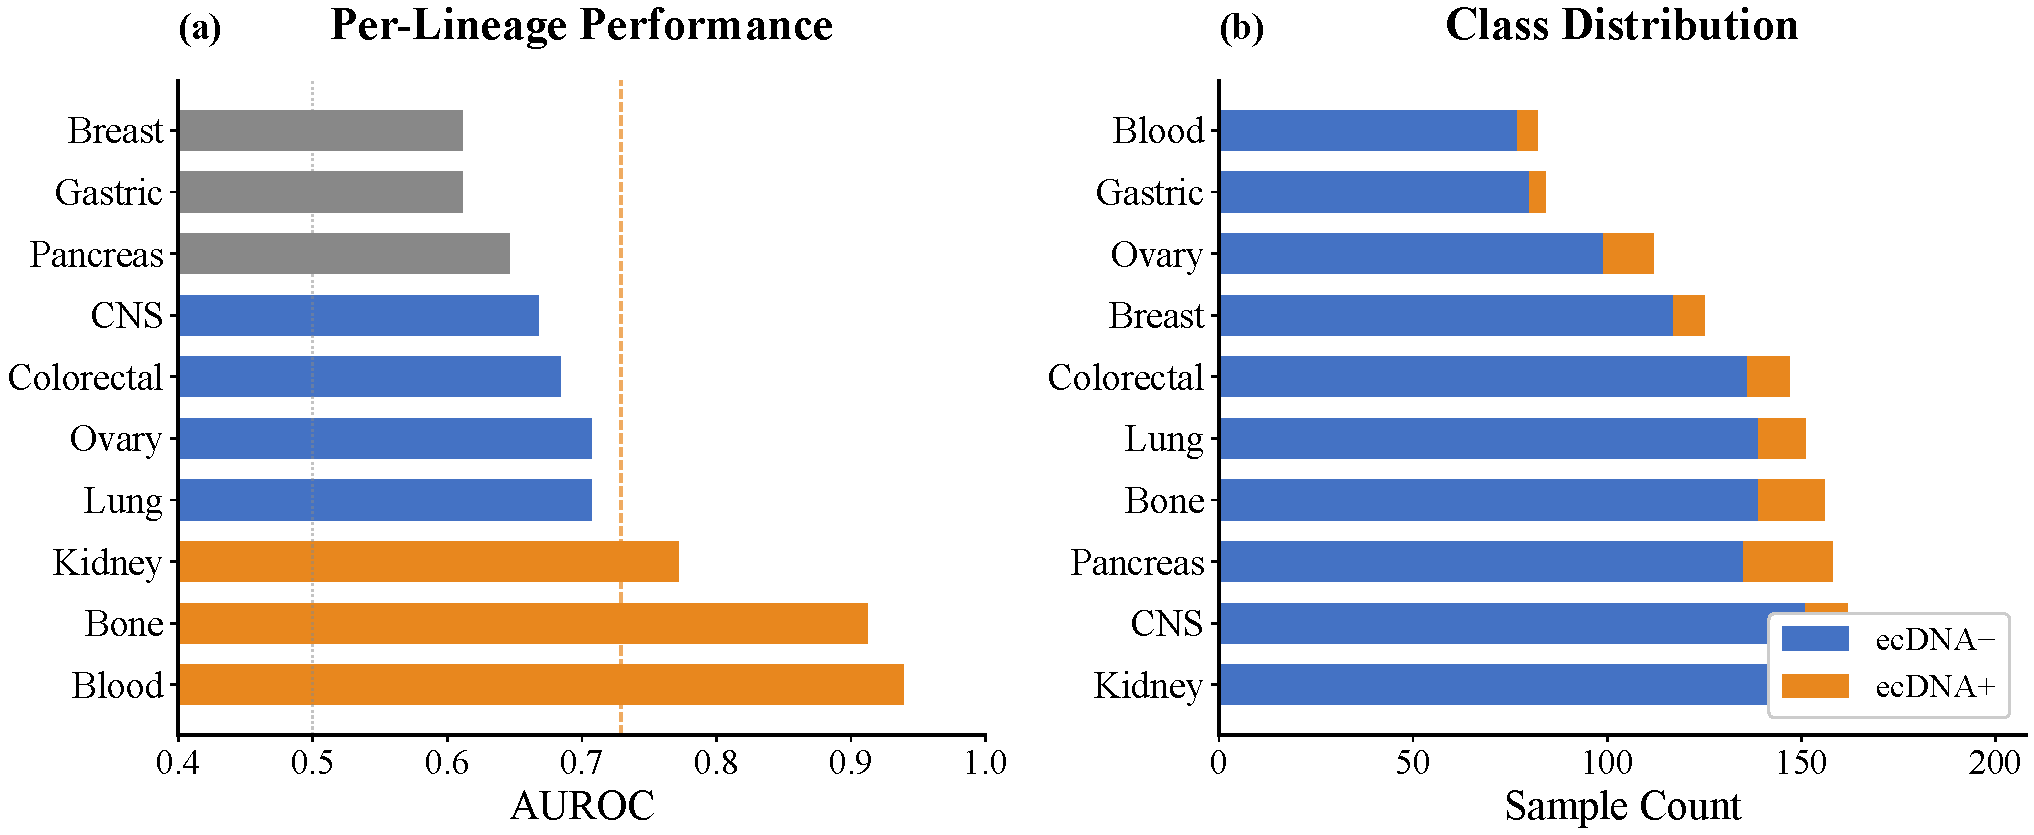
\includegraphics[width=\textwidth]{figures/fig_supp_lineage.pdf}
\caption{\textbf{Per-lineage performance analysis.} (a) AUROC by lineage. (b) Class distribution per lineage.}
\label{fig:supp_lineage}
\end{figure}

\begin{figure}[h]
\centering
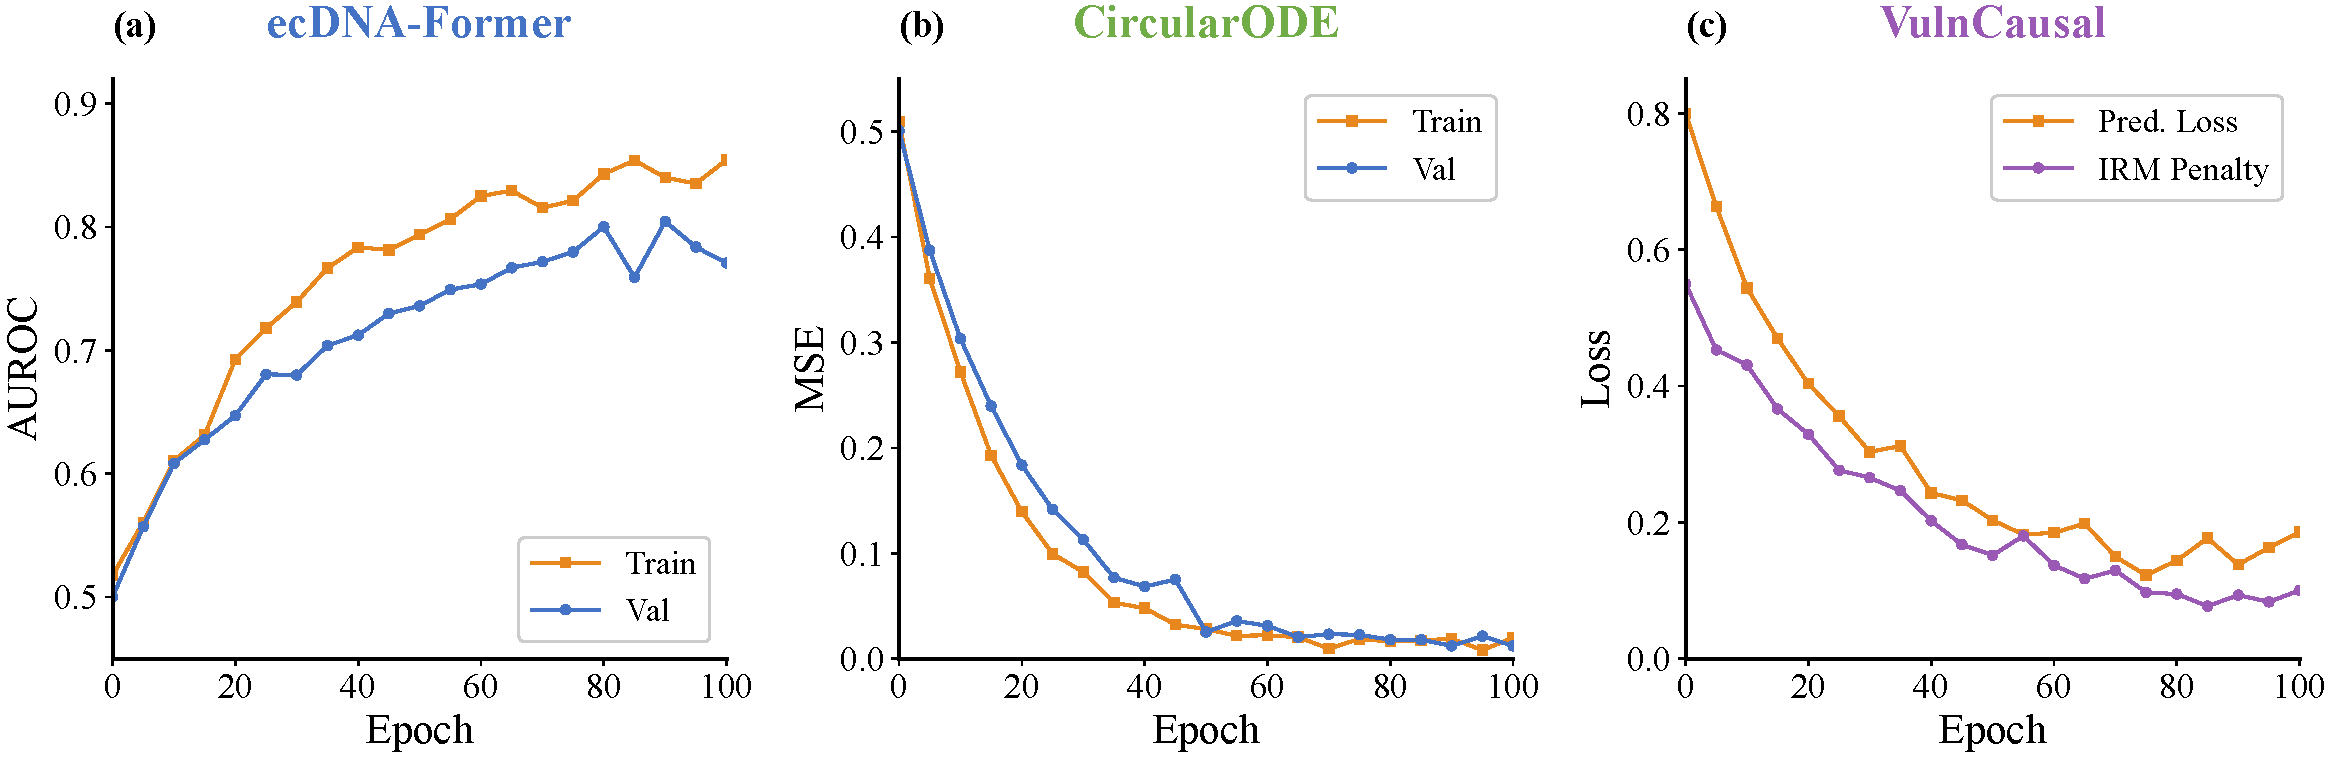
\includegraphics[width=\textwidth]{figures/fig_supp_training.pdf}
\caption{\textbf{Training dynamics for all \eclipse{} modules.}}
\label{fig:supp_training}
\end{figure}


\end{document}
